\paragraph{IUP01 Iniciar sesión}  \hspace{1cm}\\ 
\label{pant:IUP01}

\textbf{\textcolor[rgb]{0, 0, 0.545098}{Objetivo}}\\
Esta pantalla permite al Practicante iniciar sesión en la herramienta, solicitando al Practicante la información necesaria para ingresar a la herramienta.\\

\textbf{\textcolor[rgb]{0, 0, 0.545098}{Diseño}}\\
La figura \ref{fig:IUP01} muestra al Practicante los campos requeridos para iniciar sesión en la herramienta. \\

En la parte inferior se encuentra el botón Iniciar sesión para ingresar a la herramienta, además del botón  ¿Olvidaste tu contraseña o usuario? el cual muestra la pantalla \nameref{pant:IUP01.1}.

\begin{figure}[H]
	\centering
		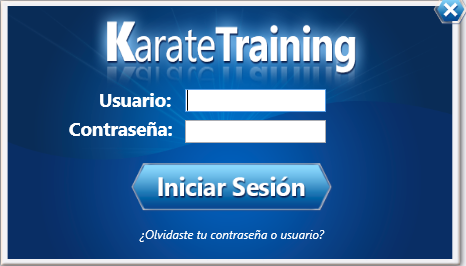
\includegraphics[scale=1]{./Figuras/Pantallas/IUP01Iniciar_sesion}
	\caption{IUP01 Iniciar sesión}
	\label{fig:IUP01}
\end{figure}

\textbf{\textcolor[rgb]{0, 0, 0.545098}{Entradas}}\\
En esta pantalla el Practicante debe capturar la siguiente información:

\begin{itemize}
	\item El nombre de usuario.
	\item La contraseña respectiva a su cuenta de usuario.
\end{itemize}

\textbf{\textcolor[rgb]{0, 0, 0.545098}{Comandos}}	%SON LOS BOTONES
\begin{itemize}
	\item \textbf{\textcolor[rgb]{0, 0, 0.545098}{Iniciar sesión:}}  Permite al Practicante iniciar sesión en la herramienta cuando la información ingresada en los campos obligatorios sea correcta. 
\end{itemize}
\vspace{1em}

\textbf{\textcolor[rgb]{0, 0, 0.545098}{Mensajes}}\\

\textbf{\nameref{msj:MSG10}}: Se muestra en pantalla , cuando el Practicante haya ingresado alguno de los datos de manera incorrecta.\\

\clearpage